\begin{appendices}
	\section{Résultats}
	\subsection{Bruteforce}\label{annexe:bruteforce}
	\begin{table}[H]
		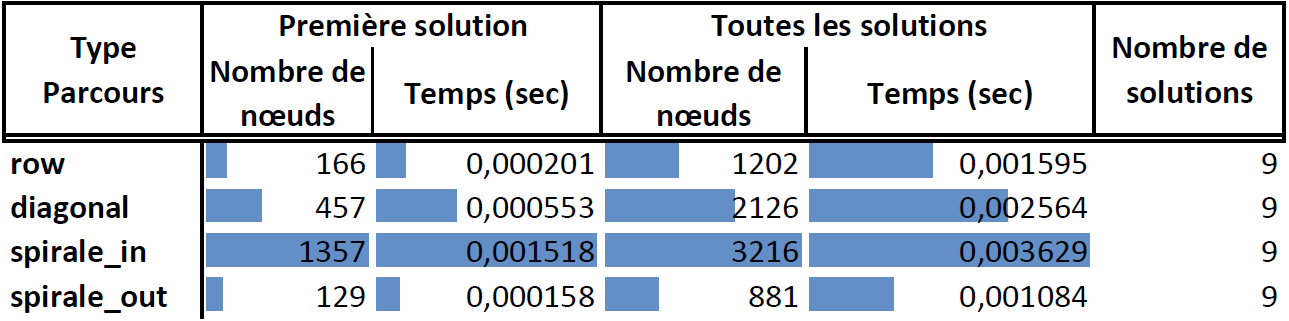
\includegraphics[width=\linewidth]{images/resultat_bruteforce_4}
		\caption{Résultats de la bruteforce pour une instance de taille 4}
	\end{table}
	\begin{table}[H]
		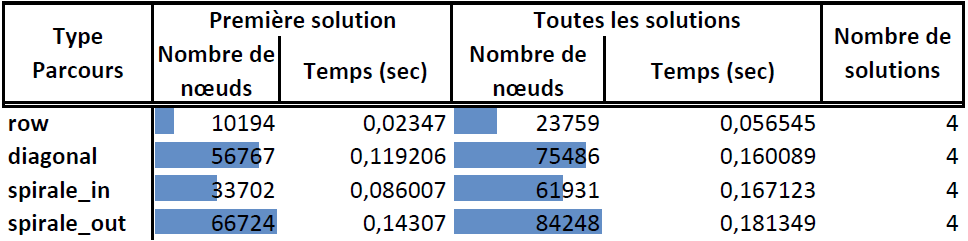
\includegraphics[width=\linewidth]{images/resultat_bruteforce_5}
		\caption{Résultats de la bruteforce pour une instance de taille 5}
	\end{table}
	\begin{table}[H]
		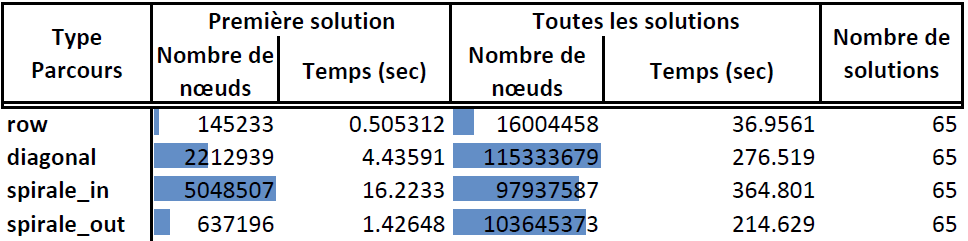
\includegraphics[width=\linewidth]{images/resultat_bruteforce_6}
		\caption{Résultats de la bruteforce pour une instance de taille 6}
	\end{table}
	
	\begin{figure}[H]
		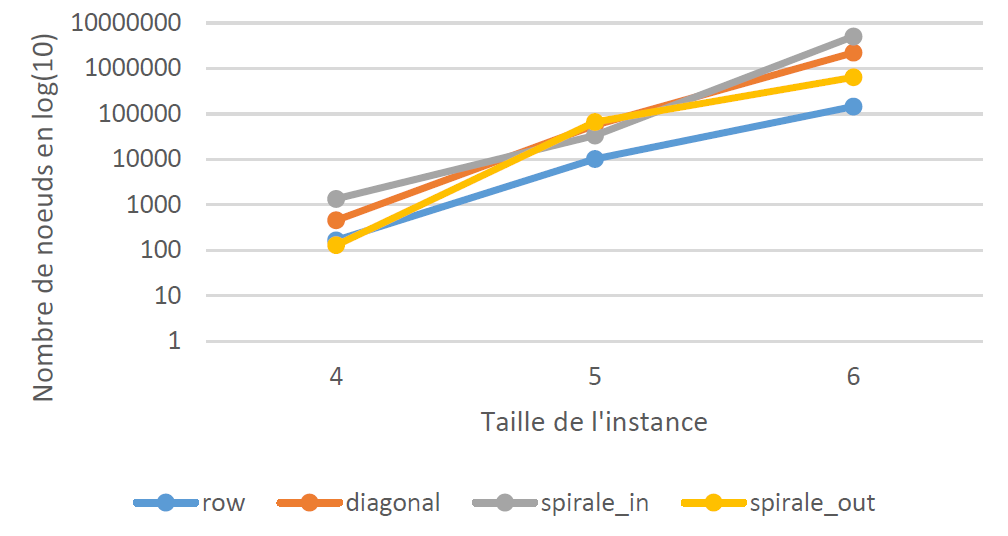
\includegraphics[width=\linewidth]{images/resultat_bruteforce_graphique_first}
		\caption{Nombre de n\oe uds à la première solution en fonction de la taille de l'instance}
		\label{fig:results_bruteforce_graphique_first}
	\end{figure}
	
	\begin{figure}[H]
		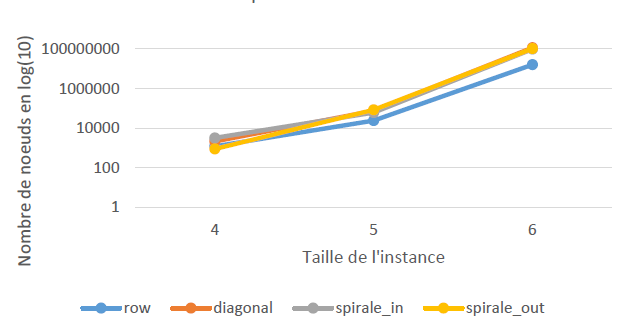
\includegraphics[width=\linewidth]{images/resultat_bruteforce_graphique_all}
		\caption{Nombre total de n\oe uds en fonction de la taille de l'instance}
		\label{fig:results_bruteforce_graphique_all}
	\end{figure}
	
	\begin{table}[H]
		\centering
		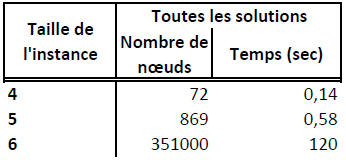
\includegraphics[width=0.6\linewidth]{images/resultat_bruteforce_rowscan_bourreau}
		\caption{Résultats de la bruteforce (rowscan) en programmation par contrainte}
	\end{table}
	
	\begin{figure}[H]
		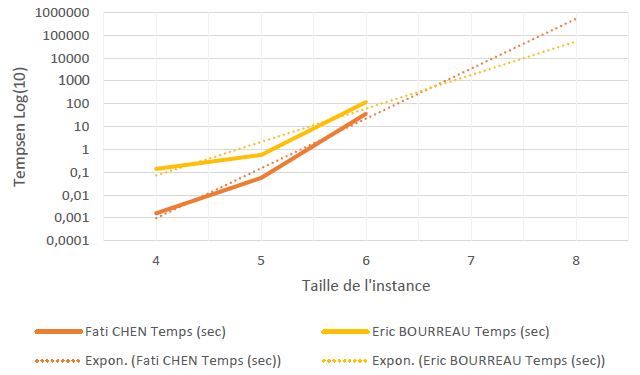
\includegraphics[width=\linewidth]{images/resultat_bruteforce_rowscan}
		\caption{Temps nécessaire au parcours complet de l'arbre}
		\label{fig:results_bruteforce_graphique_compare}
	\end{figure}

	\subsection{Smartforce}\label{annexe:smartforce}
		\begin{table}[H]
			\centering
			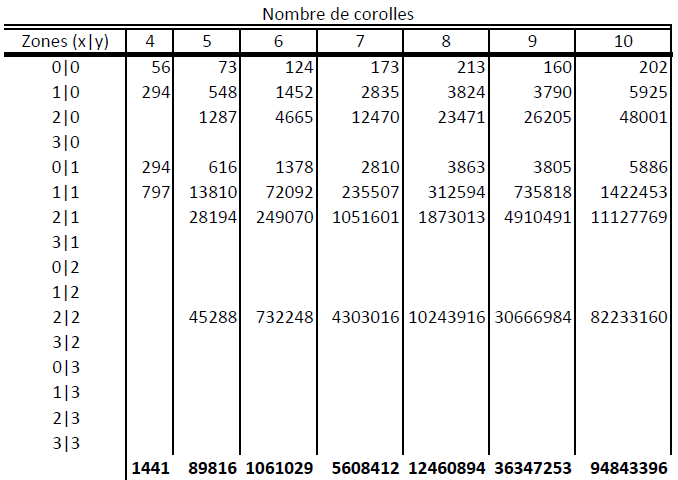
\includegraphics[width=0.8\linewidth]{images/resultats_corolle_hamming_1}
			\caption{Quantité de corolles de hamming 1 en fonction de la taille de l'instance}
		\end{table}
		
		\begin{table}[H]
			\centering
			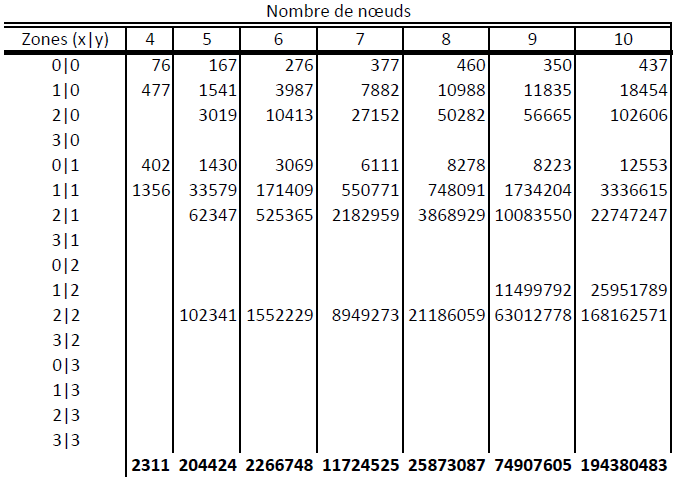
\includegraphics[width=0.8\linewidth]{images/resultats_corolle_hamming_1_noeuds}
			\caption{Nombre de n\oe uds afin de déterminer les corolles de hamming 1}
		\end{table}

		\begin{table}[H]
			\centering
			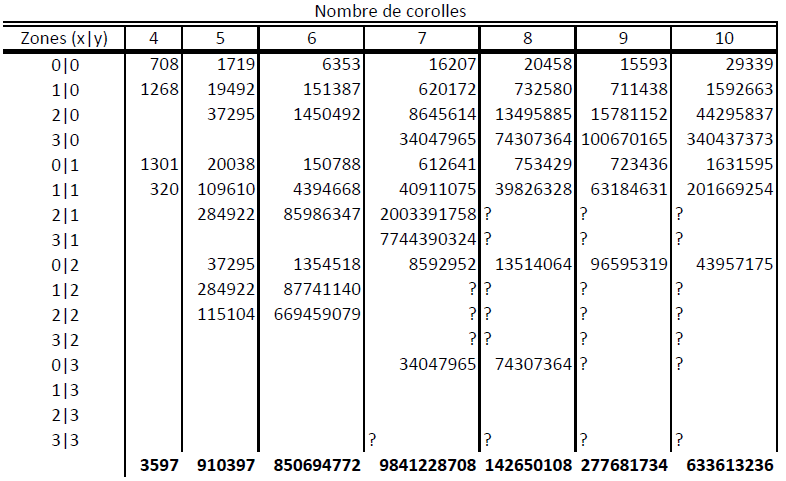
\includegraphics[width=0.8\linewidth]{images/resultats_corolle_hamming_2}
			\caption{Quantité de corolles de hamming 2 en fonction de la taille de l'instance}\label{table:count_hamming_2}
		\end{table}
		\begin{table}[H]
			\centering
			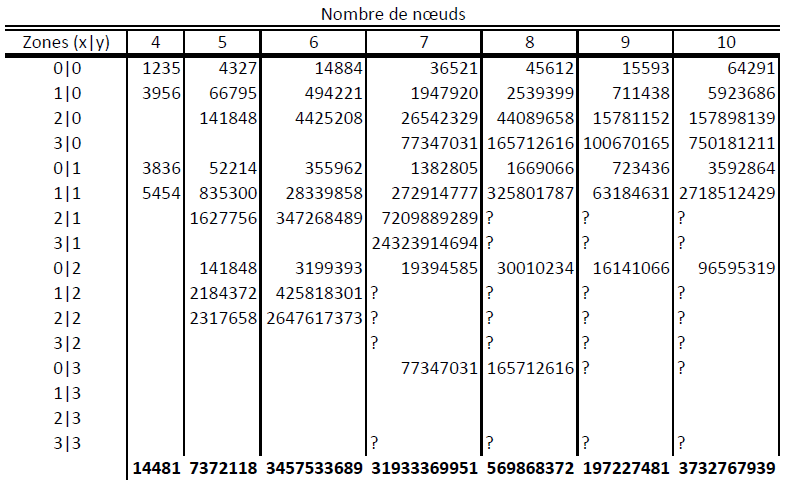
\includegraphics[width=0.8\linewidth]{images/resultats_corolle_hamming_2_noeuds}
			\caption{Nombre de n\oe uds afin de déterminer les corolles de hamming 2}
		\end{table}

	\begin{table}[H]
		\centering
		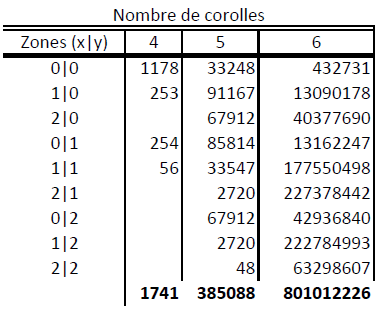
\includegraphics[width=0.6\linewidth]{images/resultats_corolle_hamming_3}
		\caption{Quantité de corolles de hamming 3 en fonction de la taille de l'instance}
	\end{table}
	\begin{table}[H]
		\centering
		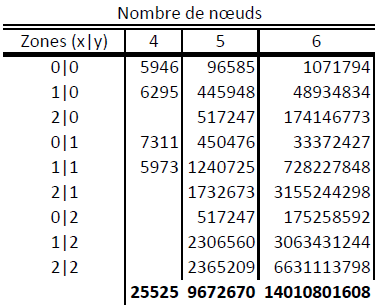
\includegraphics[width=0.6\linewidth]{images/resultats_corolle_hamming_3_noeuds}
		\caption{Nombre de n\oe uds afin de déterminer les corolles de hamming 3}
	\end{table}
\end{appendices}